% Successive time derivatives show the invariant-set mechanism.
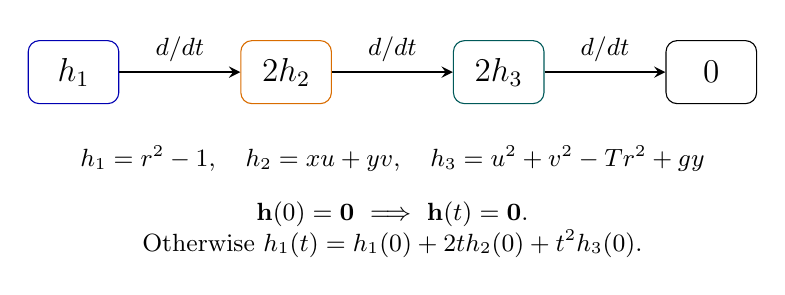
\begin{tikzpicture}[>=stealth,box/.style={draw,rounded corners,minimum width=1.15cm,minimum height=.8cm,font=\large}]
\node[box,draw=blue!70!black](a)at(0,0){$h_1$};
\node[box,draw=orange!85!black](b)at(2.7,0){$2h_2$};
\node[box,draw=teal!70!black](c)at(5.4,0){$2h_3$};
\node[box](d)at(8.1,0){$0$};
\draw[->,thick](a)--node[above,font=\small]{$d/dt$}(b);
\draw[->,thick](b)--node[above,font=\small]{$d/dt$}(c);
\draw[->,thick](c)--node[above,font=\small]{$d/dt$}(d);
\node[font=\small,align=center]at(4.05,-1.1){$h_1=r^2-1,\quad h_2=xu+yv,\quad h_3=u^2+v^2-Tr^2+gy$};
\node[font=\small,align=center]at(4.05,-2){$\mathbf h(0)=\mathbf0\ \Longrightarrow\ \mathbf h(t)=\mathbf0$.\\Otherwise $h_1(t)=h_1(0)+2t h_2(0)+t^2h_3(0)$.};
\end{tikzpicture}
